\section{Architektur und Komponenten}\label{sec:architektur-und-komponenten}

Das Evaluationsframework ist modular aufgebaut und nutzt eine Pipeline-Architektur, um wie in \hyperlink{FA02}{FA02} gefordert, eine flexible und skalierbare Evaluierung zu ermöglichen. Die Architektur ist in Abbildung~\ref{fig:evaluation-framework-architecture} dargestellt. Sie besteht aus mehreren Hauptkomponenten, die jeweils eine klar definierte Aufgabe erfüllen. Im Folgenden werden die Komponenten und ihr Zusammenspiel beschrieben.

\begin{figure}[h]
    \centering
    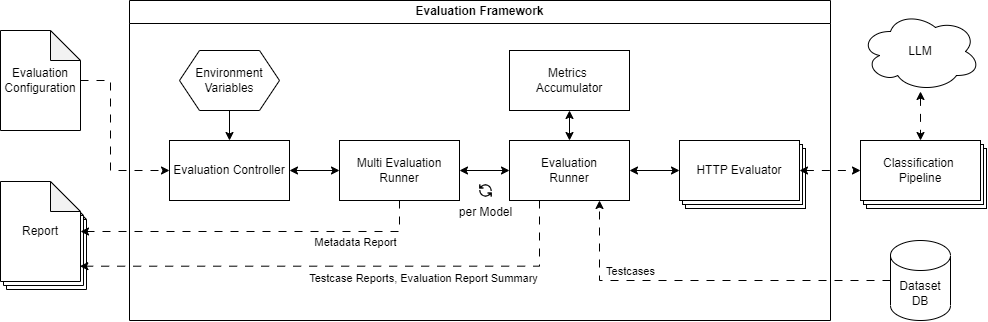
\includegraphics[width=\linewidth]{images/evaluation/evaluation-framework-architecture.drawio}
    \caption{Architektur des Evaluationsframeworks}
    \label{fig:evaluation-framework-architecture}
\end{figure}

Das Framework bietet zwei Einstiegspunkte zur Ausführung einer Evaluierung: Eine Evaluation kann mittles \texttt{EvaluationController} über einen HTTP-Request oder über die Kommandozeile über den \texttt{EvaluationCommand} gestartet werden. Beide Einstiegspunkte akzeptieren die Konfiguration aus Kapitel \ref{sec:konfiguration-einer-evaluierung}, lösen ggf.\ Umgebungsvariablen auf und delegieren die Ausführung der Evaluation an den \texttt{MultiEvaluationRunner}.

Die Architektur trennt Zuständigkeiten strikt: Der \texttt{MultiEvaluationRunner} koordiniert die Modellläufe und steuert die Anzahl der \emph{Wiederholungen} pro Modell. \texttt{EvaluationRunner} verarbeitet die einzelnen Testfälle innerhalb einer Wiederholung und sammelt Metriken. \texttt{HttpEvaluator} kommuniziert mit der Klassifizierungspipeline und der \texttt{Metrics Accumulator} aggregiert Ergebnisse pro Modell über mehrere Testfälle.